\begin{savequote}
Gesture is a critical link running through the evolution of perception,
conceptualization, and language.
\qauthor{David Armstrong, William Stokoe, and Sherman Wilcox, \textit{Gesture
and the nature of language}}
\end{savequote}
\chapter{Introduction}
% (Start with a motivating scenario: either Powerpoint presentation or USAR
% application.)
% \begin{quotation}
% \textit{Imagine an earthquake has hit a populous area and many major roads are
% impassable. Buildings are severely damaged or collapsed, and fire has broken out
% in many places. At the crisis management center, response professionals are
% working together to coordinate the earthquake relief effort. You are the
% incident commander charged with coordinating the search
% and rescue teams working in the field. There is a large tabletop display in
% front of you, showing the map of the site. Information coming from the field is
% updated on the display in real-time.}
% 
% \textit{A report about a big explosion at a chemical plant comes in and you move
% the map around, zoom in and rotate it to get a good view of the plant. On the
% map, you see there is a group of unmanned vehicles nearby. After selecting them
% on the map with your hand, you speak to the interface ``Go nearer to the
% explosion site to gather more information,'' while tracing the route the
% vehicles should take to avoid obstacles. Then you instruct rescue team No. 3 to evacuate the residents
% in the surrounding buildings by going under a bridge because the surface of the
% bridge is blocked. You gesture with one hand as the bridge and the other
% hand moving under it to emphasize this.}
% \end{quotation}
% 
% The scenario above is an example in the Urban Search and Rescue (USAR) domain.
% It shows an application of a multi-modal interface to a real-world problem. Gestures play an important part in this scenario,
% providing key information about location, method and timing of movements,
% and about spatial relationship among the objects being described.
\begin{quotation}
Imagine how nice it would be, the next time you make a presentation, if you did
not need to stand close to your laptop, or use a remote control with its limited
functionality. What if you could present your work as naturally as having a
conversation with your audience. You swipe your hand left and right to change
slides. When you point to the slide with your hand, the display shows a 
cursor following wherever you point. When you are showing a video, you use a
palm forward hand pose (``stop'' gesture) to pause the movie, then move left and
right to fast forward or rewind the video. You can also say ``faster'' or
``slower'' to change the video speed. When you need to jump to a particular
slide, you make a circle gesture to show all the slides, and say ``show this
slide'' while pointing at that slide. You can also make a dismiss gesture to
pause the slide show (making the screen black) to take the distracting slides
off the screen and get the full attention of the audience.
\end{quotation}

This scenario shows an application of a multimodal interface to a
real-world problem, with different categories of gestures playing an important
part in the scenario. The system I developed makes the scenario real
(Figure~\ref{fig:demo-circle}
and~\ref{fig:demo-point}\footnote{A live demo video can be found at
\url{https://www.youtube.com/watch?v=09BXfN2vk1E}}).
It provides real-time continuous gesture recognition and interaction, addressing problems that have previously been neglected, such as handling different types of gestures, and determining how and when the system should respond.


\begin{figure}[tbh]
\centering
\hspace{-0.6em}
\subfigure{
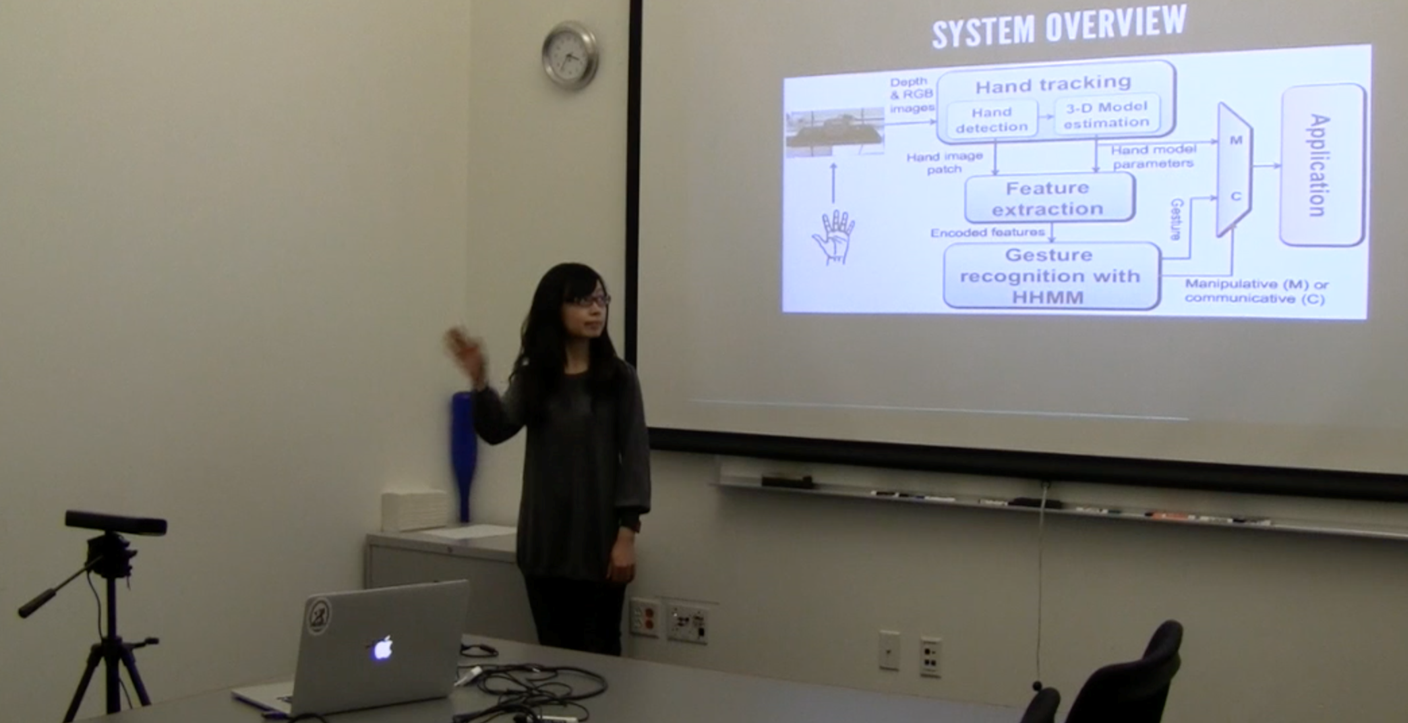
\includegraphics[width=0.33\textwidth]{figures/circle1.png}\hspace{-0.5em}}
\subfigure{
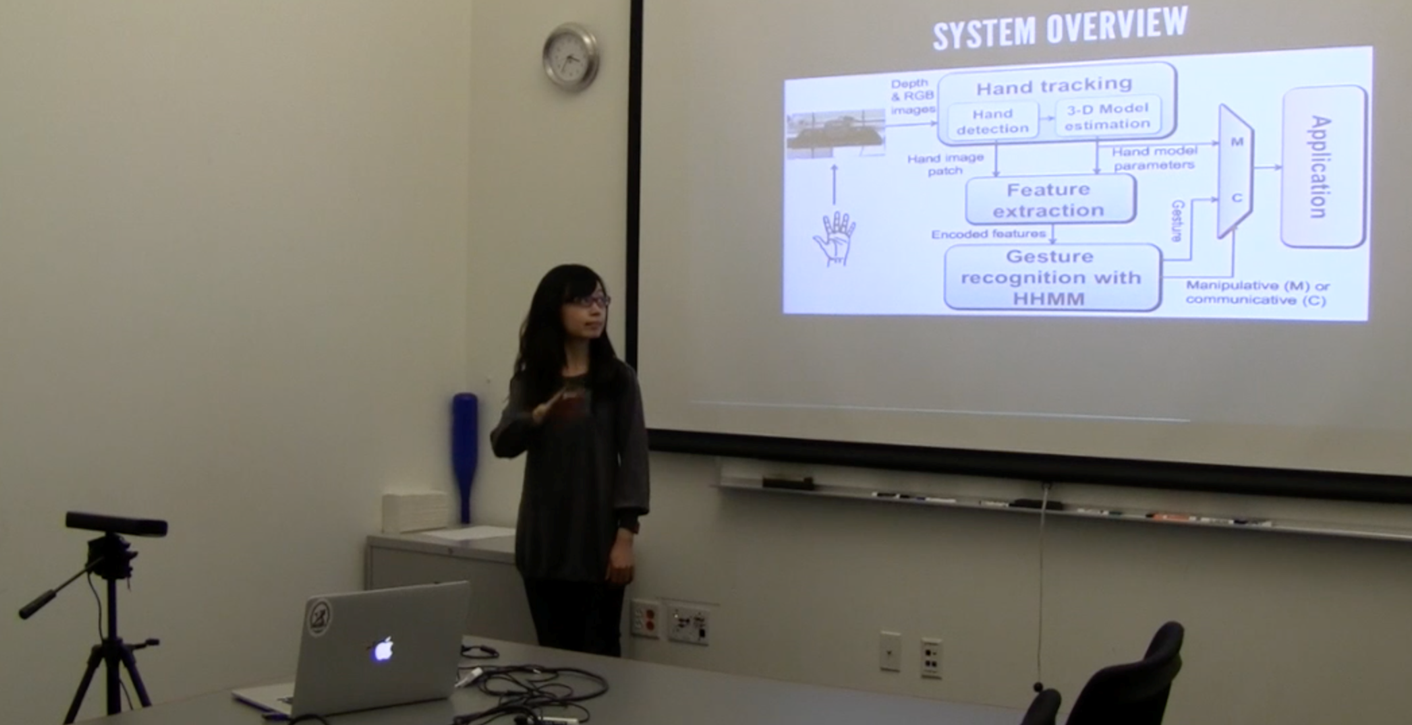
\includegraphics[width=0.33\textwidth]{figures/circle2.png}\hspace{-0.5em}}
\subfigure{
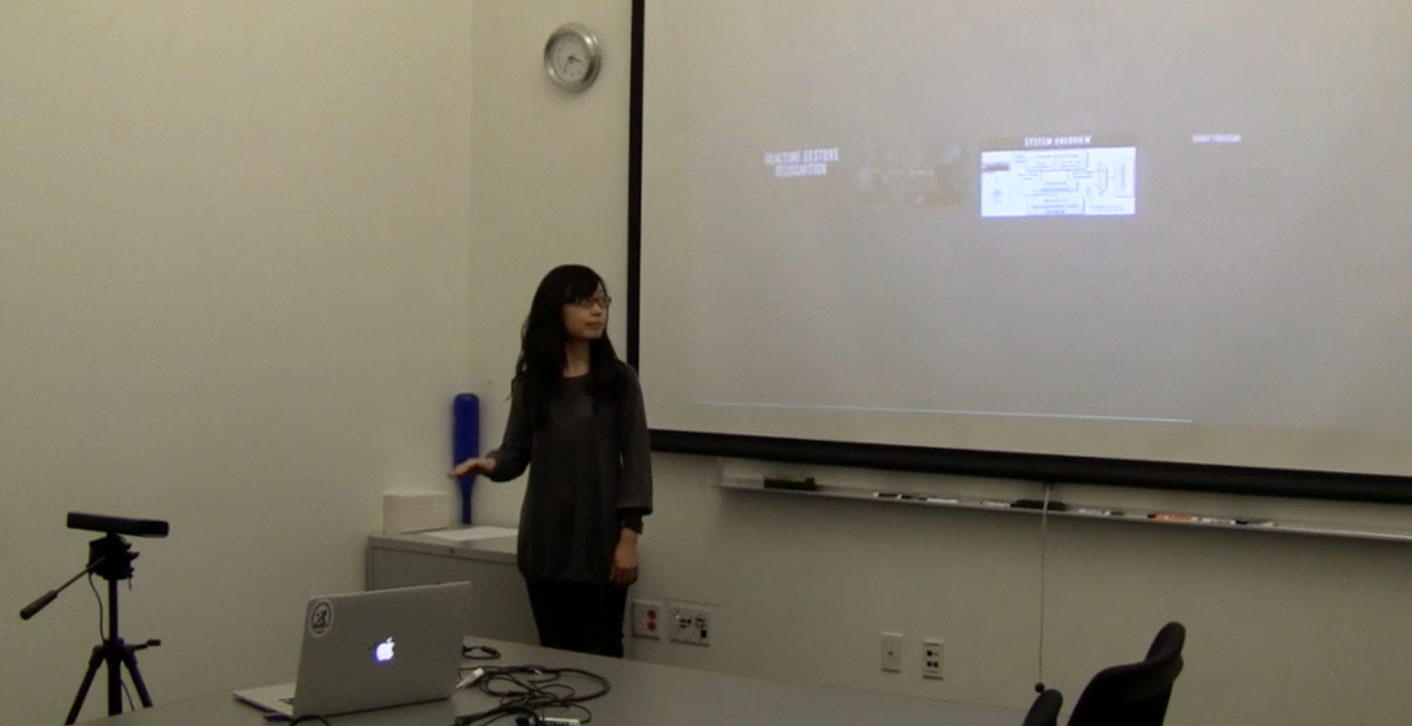
\includegraphics[width=0.33\textwidth]{figures/circle3.png}}
\caption{Real-time demonstration of the gesture controlled presentation
application. The sequence shows using a circle gesture to bring up all the
slides.}
\label{fig:demo-circle}
\end{figure}

\begin{figure}[tbh]
\centering
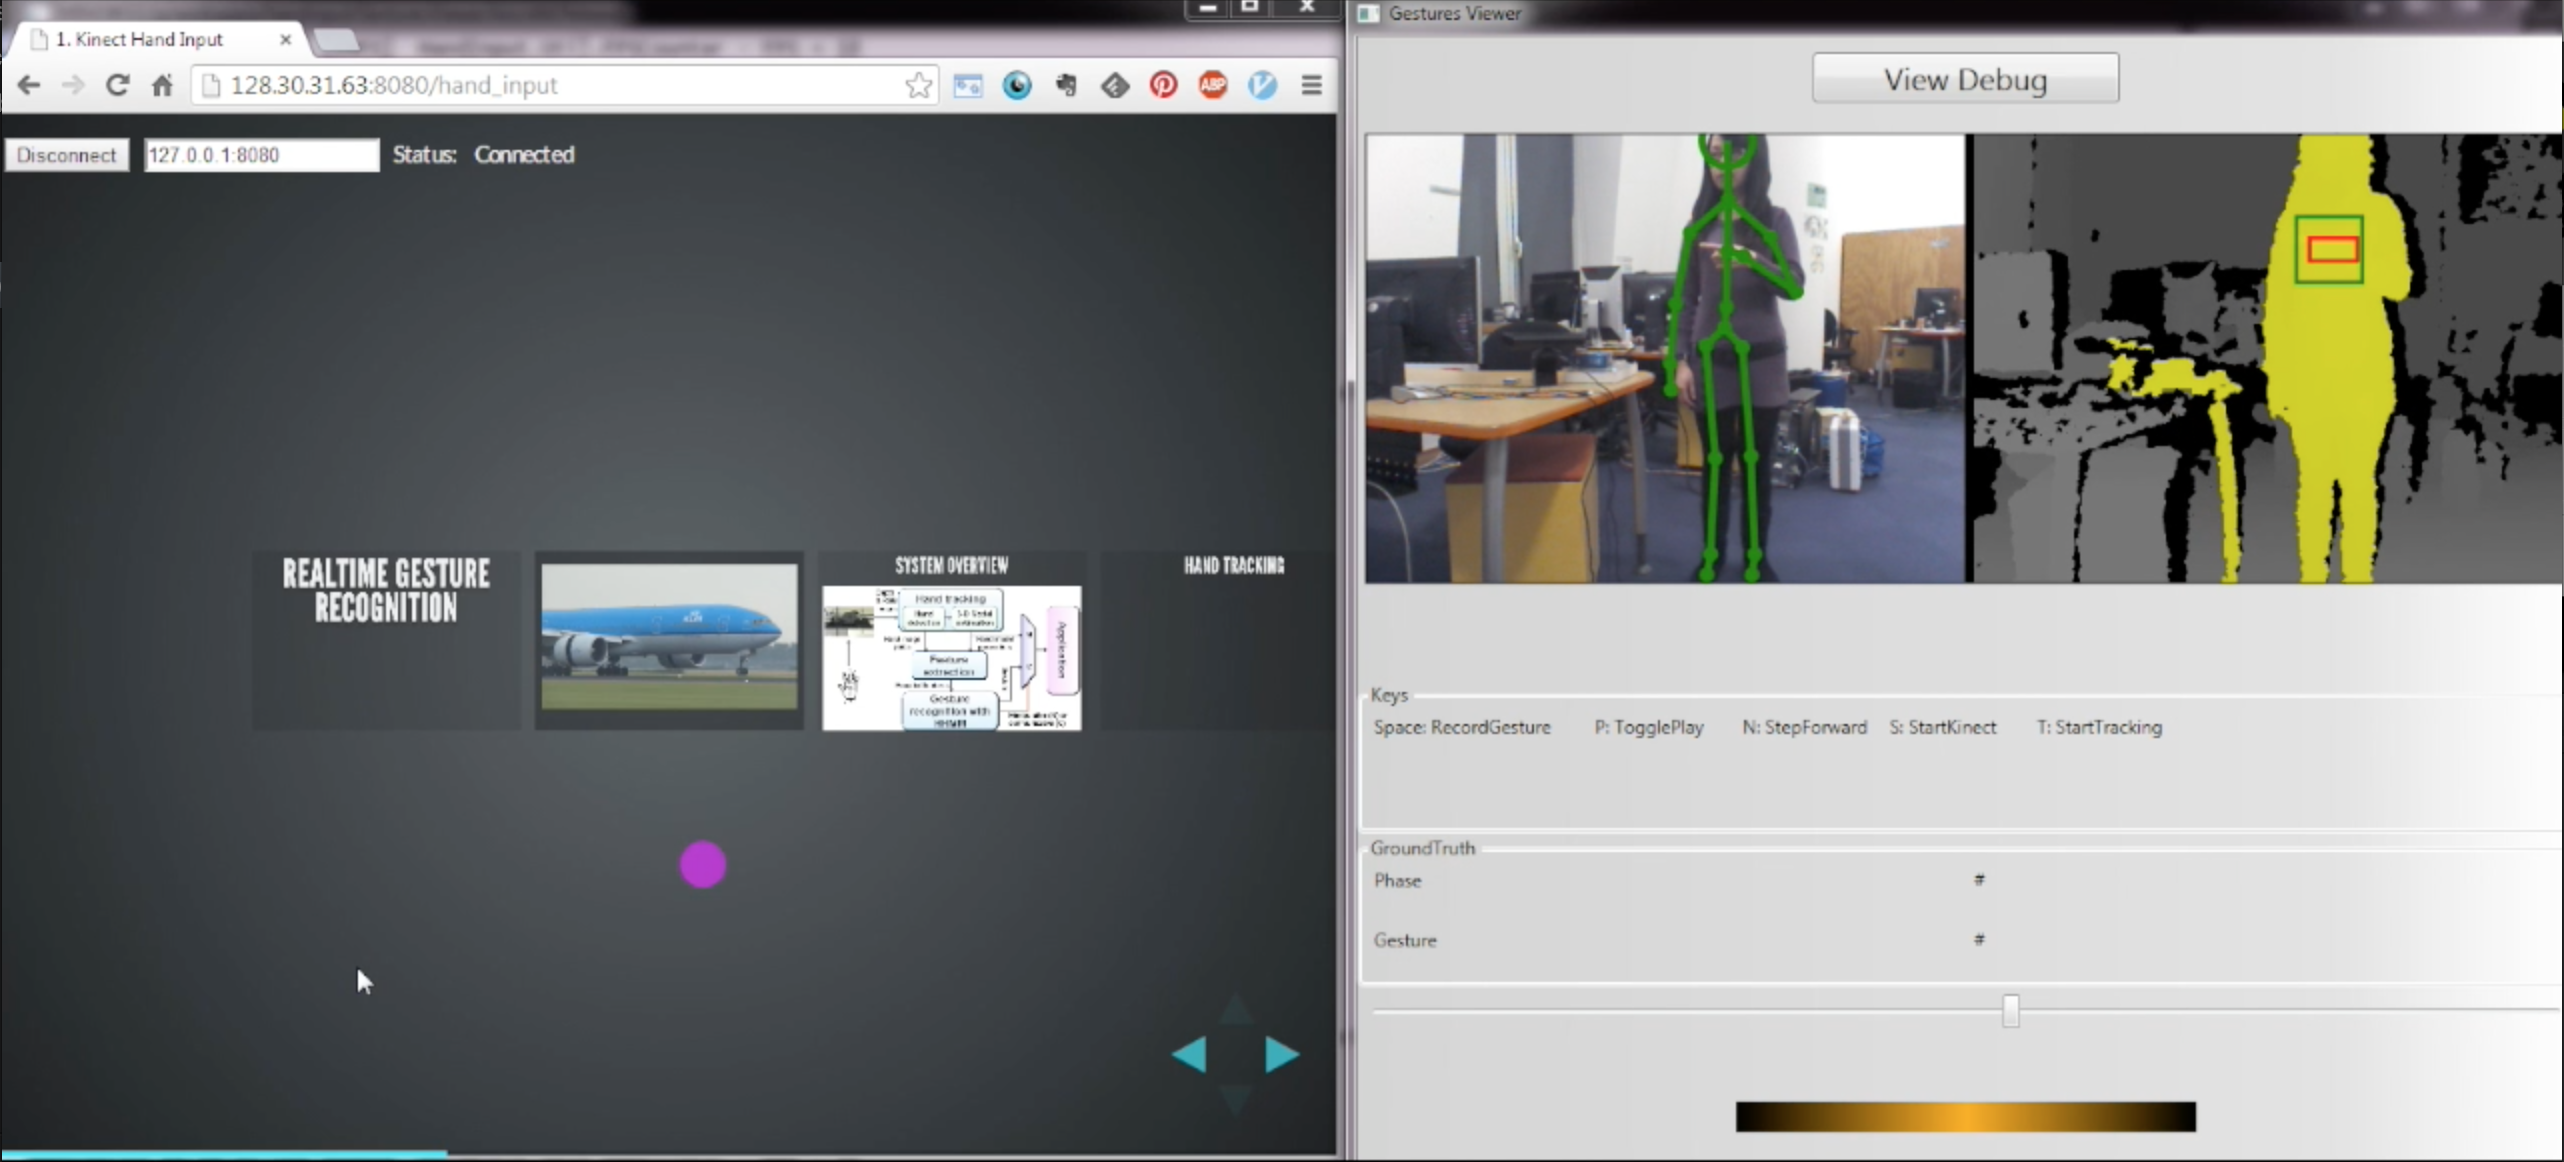
\includegraphics[width=\textwidth]{figures/point_ppt.png}
\caption{Two views of the gesture controlled presentation application. The
left view is the browser based presentation framework. The purple
circle indicates that the user is pointing at the slide. The right view is the
debug interface showing the RGB image, the depth mapped image, the skeleton
tracking, and the bounding box of the gesturing hand.}
\label{fig:demo-point}
\end{figure}
 
Recent trends in user interfaces have brought on a new wave of interaction
techniques that depart from the traditional mouse and the keyboard,
including multi-touch interfaces (e.g., the iPhone, the iPad and the Microsoft 
Surface) as well as camera-based systems (e.g., 
the Microsoft Kinect and the Leap Motion Controller). Most
of these devices gained instant popularity among consumers, and the common trait
among them is that they make interacting with computation more natural and 
effortless. Many of them allow users to use their hands and/or body 
gestures to directly manipulate virtual objects. This feels more natural 
because this is how we interact with our environment everyday.
 
There is also a trend in wearable human-computer interfaces 
(e.g., Google Glass, Samsung's Galaxy Gear smartwatches, Pebble
smartwatches) that have potential for gesture input as well. Google
Glass has a camera that can be used to recognize hand motion and hand shapes,
while the accelerometers and gyroscopes in the smartwatches can be used to
measure hand motion.

There is considerable potential and demand for natural interaction, and gesture
is an important part of it. We are starting to see more gestural
interfaces, but many of them still require that the hands function as a mouse
with a limited number of other gestures. Our goal is to break this old
paradigm of ``point, click, drag'' interaction. 
Our hands are much more versatile, and hence, offer the chance to design a
gesture recognition system for natural human computer interaction (HCI)
starting from the user interaction perspective. This means asking: what 
different types of gestures do people use; when should the system respond; how
should the model be defined and trained; and how should we combine gesture and
speech? These are the questions addressed in this thesis. Based on my
findings, I developed a real-time continuous gesture recognition and
interaction system that handles different types of gestures seamlessly, and
responds to gestures appropriately.

\section{Background}
To design a natural gesture input interface, it is important to understand the
nature of human gestures. This section gives some background on
gesture production and taxonomy, and introduces several important concepts and
terms central to the final system design.
 
\subsection{Definition of Gestures}
For a natural
interface, it is important for the system to distinguish gestures from
non-gestures (e.g., unconscious habitual movements like scratching one's head)
because this will avoid restricting how people place or move their hands when
they are not doing any purposive gestures.

Webster's Dictionary defines gestures as ``\ldots a movement usually of the body or limbs
that expresses or emphasizes an idea, sentiment, or attitude.'' This definition
is particularly related to the communicative aspect of the human hand and body
movements. However, in HCI, the notion
of gestures is somewhat different. In their review of the visual interpretation
of hand gestures for HCI, Pavlovi\'{c} et al. \cite{Pavlovic97} state that in a
computer controlled environment one wants to use the human hand to perform tasks that
mimic the natural use of the hand both as a manipulator and as used in
human-machine communication. They describe this in part by having both
\textit{manipulative} and \textit{communicative} gestures in their gesture taxonomy. We adopt this
distinction.

\begin{figure}[tbh]
  \centering
  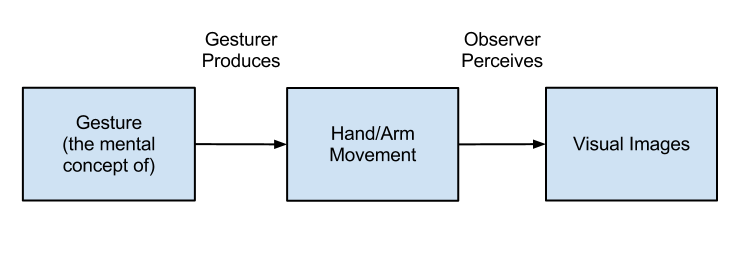
\includegraphics[width=0.7\textwidth]{figures/gesture_production.png} 
  \caption{Production and perception of gestures. Hand gestures originate as a
  mental concept, are expressed through arm and hand motion, and are perceived
  as visual images \cite{Pavlovic97}.}
  \label{fig:gesture_production}
\end{figure}

Pavlovi\'{c} et al. \cite{Pavlovic97} also gives a model (Figure. 
\ref{fig:gesture_production}) for the production and perception of gestures, 
based on the model used in the field of spoken language recognition. According 
to their model, gestures originate as a gesturer's mental concept, possibly in 
conjunction with speech. They are expressed through the motion of arms and 
hands, while observers perceive gestures as streams of visual images that they
interpret using their knowledge about those gestures. In HCI, the 
observer is the computer and the knowledge it possesses is the training data.

\subsection{Gesture Taxonomy for Natural Interaction}\label{sec:taxonomy}
Several gesture taxonomies have been suggested in the literature. Some of them
deal with psychological aspects of gestures \cite{kendon86, mcneill82}, while
others are inspired by an HCI perspective \cite{Pavlovic97, quek95, wobbrock09}. 
The taxonomy that seems most appropriate for natural HCI and human-centric
design is developed by Wobbrock et al.~\cite{wobbrock09}. Their study was based
on eliciting natural behavior from non-technical users when interacting with a computing system.
As their study focused on tabletop gestures, I further generalized their
taxonomy to encompass interaction for both vertical and horizontal interfaces.

Wobbrock et al. \cite{wobbrock09} classified gestures along four
orthogonal \textit{dimensions}: \textit{form},
\textit{flow}, \textit{binding}, and \textit{nature}. Within each
dimension, there are multiple \textit{categories}, shown in
Figure~\ref{fig:taxonomy}.
The \textit{form} dimension is particularly relevant for gesture recognition
because it concerns the visual characteristics of gestures.
The \textit{flow} and the \textit{binding} dimensions are relevant for the
application layer because they are related to how the user interface (UI) should
respond to gesture events. The \textit{nature} dimension is very similar to the
taxonomies mentioned in other related work, and hence, will be explained further
below. However, the \textit{form} and the \textit{flow} dimensions are the focus
of this thesis.
Since these four dimensions have specific meanings in this taxonomy, I will refer them in italic text in the thesis to make the distinction.

\begin{figure}[tbh]
  \centering
  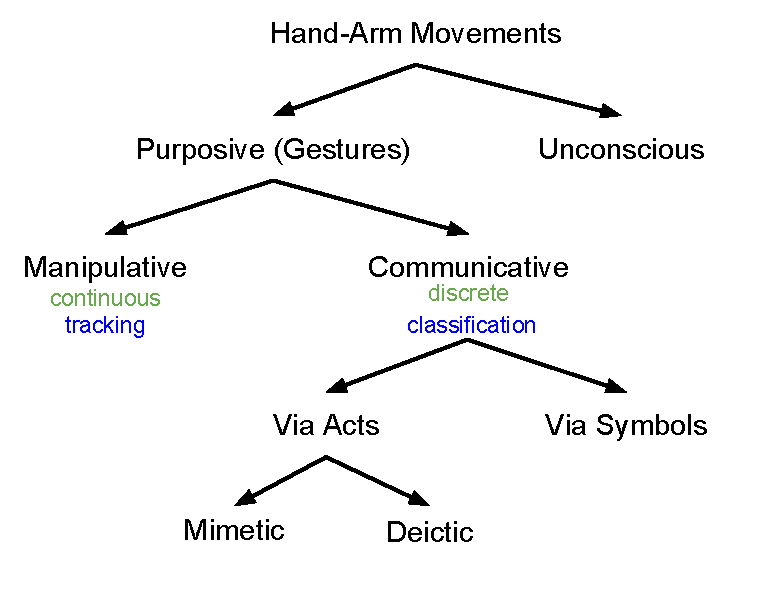
\includegraphics[width=\textwidth]{figures/taxonomy.pdf} \caption{Gesture taxonomy along
  four dimensions. The abbreviation ``w.r.t'' means ``with respect to.''}
  \label{fig:taxonomy}
\end{figure}

\subsubsection{Wobbrock's Nature Dimension}
Along the \textit{nature} dimension, Wobbrock et al. divide gestures into four
categories: symbolic, physical, metaphorical and abstract. These
categories have some overlap with Pavlovi\'{c}'s classification, but
Pavlovi\'{c}'s is more comprehensive. 

The hierarchical
categorization along the \textit{nature} dimension in Figure~\ref{fig:taxonomy}
is the one I summarized based on Pavlovi\'{c}'s taxonomy.
Gestures are divided into manipulative and communicative. Manipulative gestures are used to act on objects (e.g.
moving an virtual object around, click a button), while
communicative gestures have an inherent purpose for communication \cite{Pavlovic97}. 

People perform communicative gestures via acts or symbols. Gestures via acts are
those directly related to the interpretation of the movement itself. Such
movements are classified as either mimetic (which imitate some actions) or
deictic (pointing acts that select objects by location).
Gestures via symbols are those that have a linguistic role, and are often represented by different static hand postures. An example is forming the
O.K. pose for ``accept''. 

\subsubsection{Form and Flow Dimensions}
Although the classification in the \textit{nature} dimension gives us a good
understanding of gestures, it is less useful for designing the gesture
recognition system than the \textit{form} and the \textit{flow} dimensions are.

% \begin{table}[tbh]
% \centering
% \begin{tabular}{|c|l|l|}
% \hline
% \multirow{2}{*}{\textbf{\textit{Form}}} & \textit{distinct path} & with any hand
% pose
% \\
% \cline{2-3} 
%                                & \textit{distinct hand pose} & with any path \\
% \hline
% \multirow{2}{*}{\textbf{\textit{Flow}}} & \textit{discrete} & response occurs
% \textit{after} the user acts \\
% \cline{2-3}
%               & \textit{continuous} & response occurs \textit{while} the user
%               acts \\
% \hline
% \end{tabular}
% \caption{Gesture forms and flows.}
% \label{tab:taxonomy}
% \end{table}

I distinguish two
categories in the \textit{form} dimension: \textit{path} and \textit{pose}. The
path category contains gestures characterized by distinct paths without any distinct
hand poses. For example, a Swipe Left gesture is characterized by a
right to left motion, while a Circle gesture is characterized by a
circular motion of the hand (Figure~\ref{fig:path-gestures}). In doing these,
users typically hold their hands in some natural, relaxed, but unpredictable pose. 

\begin{figure}[tbh]
\centering
\subfigure[Swipe Left]{
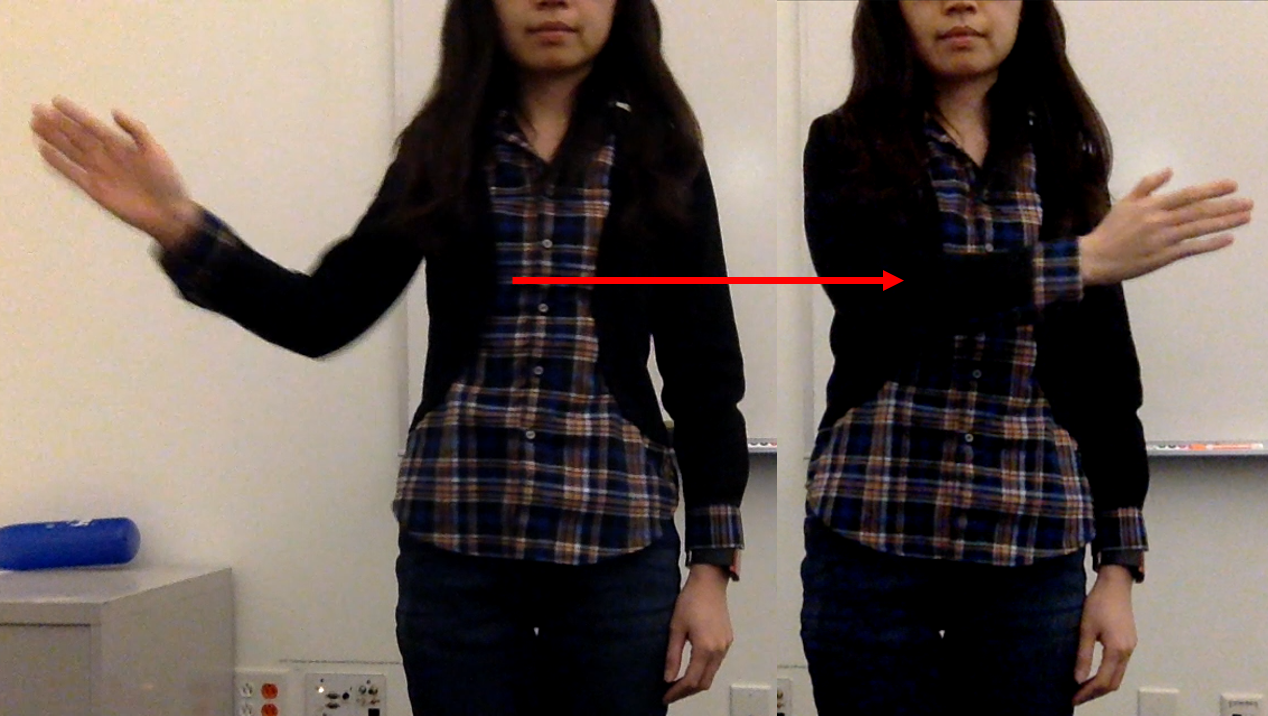
\includegraphics[width=0.6\columnwidth]{figures/swipe_left.png}
}
\subfigure[Circle]{
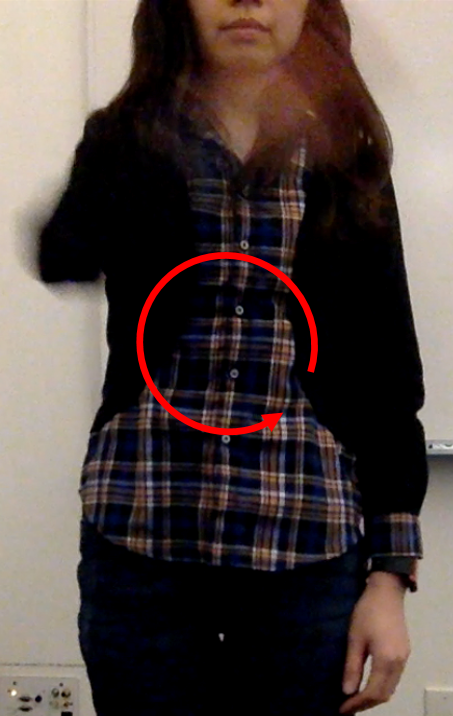
\includegraphics[width=0.215\columnwidth]{figures/circle.png}}
\caption{Examples of path gestures.}
\label{fig:path-gestures}
\end{figure}

Pose
gestures are characterized by distinct hand poses without any distinct paths.
This category of gestures is usually associated with direct manipulation of some virtual
objects on the interface.
For example, a user may use a Point hand pose and move around to
point at different things on a display.

In the \textit{flow} dimension, a gesture's flow is
\textit{discrete} if the gesture is performed, delimited, recognized, and
responded to as an atomic event~\cite{wobbrock09}. For example, if the Wave gesture is
regarded as a discrete flow gesture, the system should respond once, at the last
repetition of the left-right motion. Flow is \textit{continuous} if ongoing
recognition is required and the system should respond frame by frame, as for example during a ``point'' gesture, where we want to show the cursor on the screen
continuously moving according to the hand position. 

The \textit{form} dimension informs us what different features we need to
consider to differentiate gestures.
The \textit{flow} dimension informs us how the system should respond to gesture
events. As a result, I focus on these two dimensions in this thesis. 

While for
some gestures, their categorization along certain dimension is obvious; for
others, it is not, and the actual categorization can be decided by the
application developer or the user. Figure~\ref{fig:flow-form} shows an example
of gesture categorization along the two dimensions.

\begin{figure}[tbh]
\centering
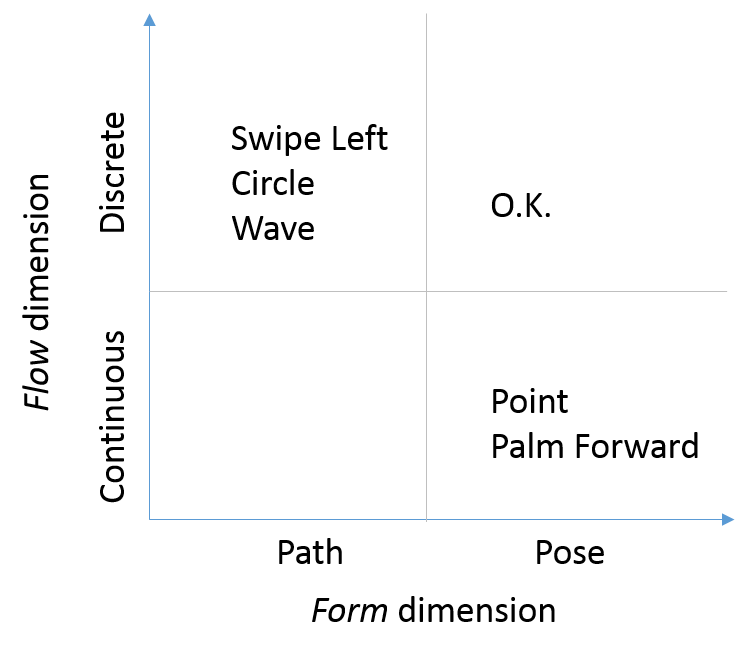
\includegraphics[width=0.6\textwidth]{figures/flow_form.png}
\caption{A categorization of gestures along the \textit{flow} and the
\textit{form} dimensions.}
\label{fig:flow-form}
\end{figure}

\subsection{Temporal Modeling of Gestures}\label{sec:temporal-model}
Making gesture interaction feel natural requires a system that responds at the
correct moment, meaning that we have to consider the temporal
characteristics of a gesture. We set a foundation for doing this by taking
account of the three \textit{phases} that make up a gesture:
\begin{itemize}
  \item pre-stroke,
  \item nucleus (peak \cite{mcneill82}), and
  \item post-stroke \cite{Pavlovic97}.
\end{itemize}
Pre-strokes and post-strokes are movement from and to the
rest position. The nucleus of a gesture,
as Kendon \cite{kendon86} observes, has some ``definite form and enhanced dynamic
qualities''. Every gesture must have a nucleus, which is the content-carrying
part of the gesture. Based on this theory, the lack of a nucleus phase can
be used to distinguish unintentional movements from gestures .

Even though the end of the
post-stroke phase can be more easily detected by finding the start of the
rest position, I want to do more than this. Since the nucleus phase is the
meaningful part of the gesture, for a discrete \textit{flow} gesture, the
system should respond immediately at the end of the nucleus, instead of at the
end of the post-stroke. To make the system more responsive, I address this challenging problem of distinguishing the start and end of the
 nucleus phase from the pre-stroke and post-stroke phases. This also allows the system to respond to continuous
\textit{flow} gestures immediately at the start of the nucleus phase.

\section{System Overview and Thesis Outline}
The gesture interaction system consists of four modules: hand tracking, 
feature extraction, gesture recognition, and application user interface
(Figure~\ref{fig:overview}). At each time frame, the
hand tracking module takes raw data from the sensor and estimates the location
of the gesturing hand. The feature extraction module computes feature
descriptors from the localized hand and sends the encoded features to the
gesture recognition module.
The gesture recognition model estimates the current most likely gesture label and gesture phase information based on the input stream of
feature vectors. The gesture information, 
together with smoothed hand position information are sent to the application
level. 

\begin{figure}[tbh]
\centering
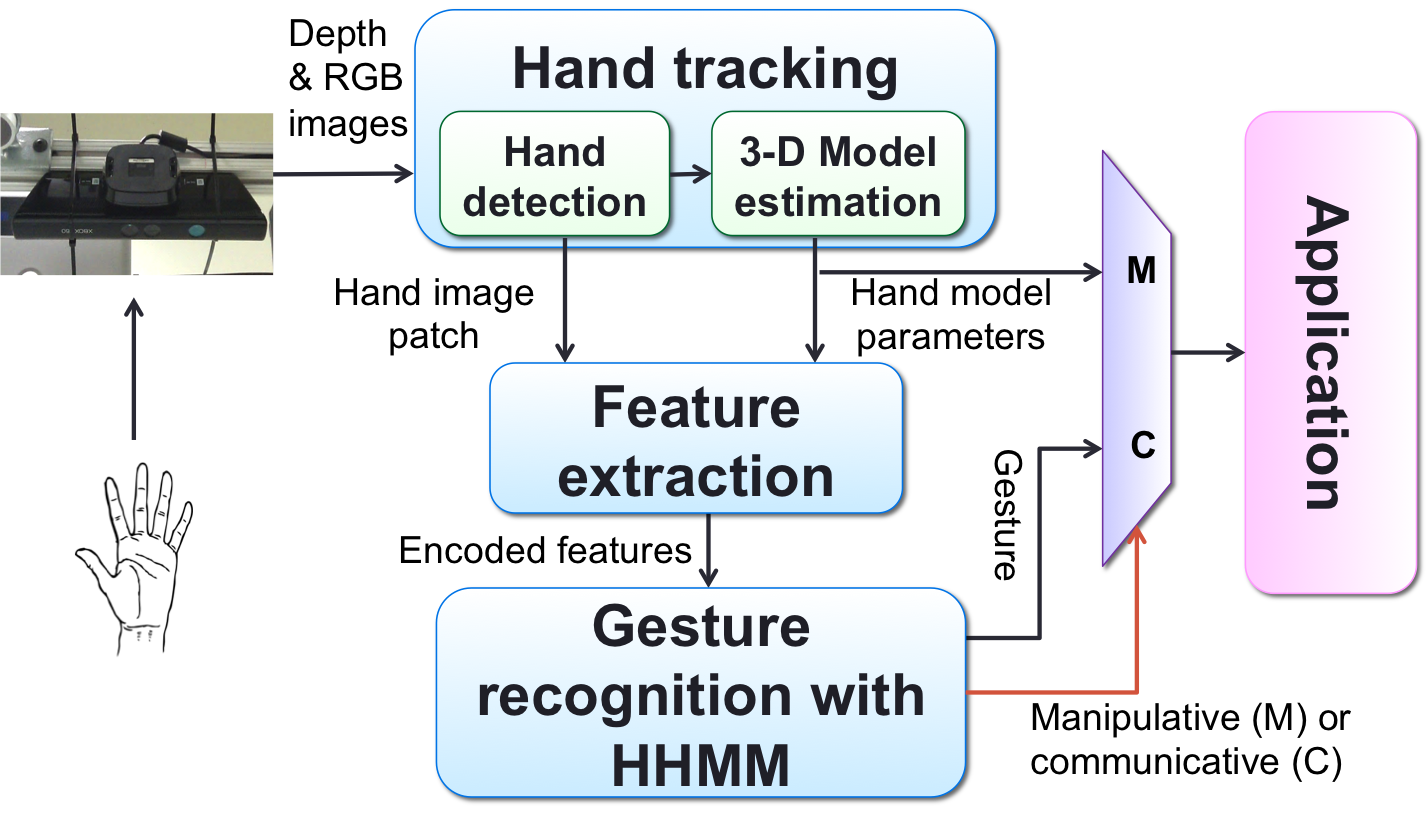
\includegraphics[width=0.7\linewidth]{figures/system_overview.png}
\caption{System overview.}
\label{fig:overview}
\end{figure}

In each module, I have developed new
techniques to improve the gesture recognition accuracy and user experience, and
improved upon existing methods.
The main focus and contributions of this work are in gesture recognition.

\section{Contributions}
The main contributions of this work include:
\begin{itemize}
 \item Hand tracking
  \begin{itemize}
  \item I improved hand tracking by replying in part on gesture salience: I
  define gesture salience to be proportional to the amount of motion and the closeness
  of the motion to the observer. Based on this, I compute a probability map for
  the gesturing hand locations in a frame.  Compared with using the hand joint
  position from the Kinect SDK, using our hand tracking method gives a 2.7\%
  absolute increase in the recognition $F_1$ score.
  \end{itemize}
 \item Feature extraction
  \begin{itemize}
  \item I use histogram of oriented gradients (HOG) as a hand shape descriptor
  and apply principal component analysis (PCA) to reduce its dimensionality. I
  then use it as part of the feature vector input to the hidden Markov models
  (HMMs) based recognition module. This novel approach allows the system to
  handle path and pose gestures in a unified way.
  \end{itemize}
  \item Gesture recognition
    \begin{itemize}
    \item I developed a probabilistic framework based on HMMs for real-time
    continuous (i.e., unsegmented) gesture recognition that unifies recognition
    of two \textit{forms} of gestures (path and pose). I use different HMM
    topologies for different forms of gestures and combine them into one
    flattened HMM for simultaneous recognition and segmentation.  With user dependent
    training and testing, the system achieves an average $F_1$ score of 0.805
    on the YANG dataset.
    \item I used embedded training and hidden state information to detect
    different gesture phases -- the pre-stroke, the nucleus, and the post-stroke
    phases -- allowing the system to respond more appropriately and promptly to
    gestures that require a discrete response and those needing a continuous
    response. With user independent training and testing on the ChAirGest
    dataset, this method achieves a temporal segmentation rate of 0.923 for
    identifying the start and the end of nucleus phases.
    \item I collected a new dataset (YANG dataset) that includes 4 path and discrete flow gestures and 3 pose and
    continuous flow gestures from 10 users), a combination currently
    lacking in the community, to evaluate system performance.
    \item I developed a hybrid evaluation metric that is more relevant to
    real-time interaction with different gesture \textit{flows}.
    \item I used gesture phase information to do gesture spotting, filtering out
non-gestures with no nucleus phases.
  \end{itemize}
  \item User interaction techniques
  \begin{itemize}
  \item I identified two main ways of combining gesture and speech for natural
  interaction: using gestures to augment speech, and using speech to augment
  gestures, and demonstrated the combination in an interactive system.
  \end{itemize}
\end{itemize}